%%% Preambolo del documento %%%
% Non toccate questa roba, a meno che non siate abbastanza sgamati da sapere quello che state facendo, tipo vi piacciono di più certi pacchetti rispetto ad altri, o magari ve ne manca qualcuno.
\documentclass[a4paper, titlepage]{article}
\usepackage[T1]{fontenc} %
\usepackage[utf8]{inputenc} %utf8x se non va utf8
\usepackage[italian]{babel} %lingua usata nel documento
\usepackage{amsmath}
\usepackage{natbib}
\usepackage{listings}
\usepackage{textcomp}
\usepackage{multirow}
\usepackage{multicol}
\usepackage{booktabs}
\usepackage{graphicx}
\usepackage{floatflt}
\usepackage{epsfig}
\usepackage{pstricks}
\usepackage{subfigure}
\usepackage[labelfont=bf, font=scriptsize]{caption}
\usepackage[italian]{varioref}
\usepackage[suftesi]{frontespizio}
\usepackage{color}
\usepackage{tikz}
\usepackage{caption}
\usepackage{pgfplots}
\usepackage[a4paper, margin=1.1in]{geometry}
\usepackage{comment}
\usepackage{lipsum}
\pgfplotsset{compat=1.16}
%%% Il documento vero e proprio %%%
\begin{document}

%%% Frontespizio %%%
% Questa serie di comandi genera il frontespizio della relazione.
% Cambiate: l'Anno Accademico, Data e Titolo della relazione, il nome degli appartenenti al gruppo con annessa matricola e mail istituzionale. Se siete due o quattro in gruppo, basta togliere/inserire una riga Candidato.
% NON toccate i comandi con accanto con CTT (Can't Touch This).
% !!! NOTA PER LA CORRETTA VISUALIZZAZIONE DEL FRONTESPIZIO. !!!
% Quando si compila un file su Overleaf, per velocizzare le successive compilazioni questi genera una cache, e da questa prende gli elementi che, a senso suo, non sono cambiati nel testo. Quindi per quanto vi possiate ostinare a compilare, vedrete sempre il primo frontespizio che ha compilato (quello con NomeCognome etc etc) e non le ultime modifica.
% Come evitare ciò, e visualizzare il frontespizio con i vostri nomi, cognomi e numeri matricola? Così: cliccate sull'icona accanto a Recompile, quella con il simbolo del documento, e successivamente sul simbolo del cestino (Clear cached files). Liberate la cache, modificate il frontespizio, e ricompilate. Così dovreste riuscire a vedere nel file compilato le vostre modifiche al frontespizio. Ricordatevi di svuotare la cache del file Overleaf ogni volta che volete modificare qualcosa nel frontespizio.
\begin{frontespizio}
%\Universita{Politecnico di Milano}
\Istituzione{Politecnico di Milano} % CTT
\Logo{Figure/logo polimi} % CTT
\Divisione{Progetto di Reti Logiche} % CTT
\Corso[Laurea Triennale]{Ingegneria Informatica} % CTT, a meno che non cambi la denominazione del corso
\Annoaccademico{2020-2021}
\Titoletto{Relazione di progetto} % CTT
\Titolo{Equalizzatore d'immagine}
\Sottotitolo{Febbraio 2021}
\NCandidati{\textbf{Gruppo di lavoro}\vspace{2.5mm}} % CTT

\Candidato{Pietro Bernardelle, \textsf {pietro.bernardelle@mail.polimi.it}\\{\small Codice Persona: 10618579}\vspace{1.5mm}}
\Candidato{Stefano Civelli, \textsf {stefano.civelli@mail.polimi.it}\\{\small Codice Persona: 10628574}}

\NRelatore{\textbf{Docenti}\vspace{2.5mm}}{} % CTT
\Relatore{Prof. William Fornaciari\\Prof. Federico Terraneo} % CTT, a meno che non sia cambiato il Prof.

\end{frontespizio}
\IfFileExists{\jobname-frn.pdf}{}{%
\immediate\write18{pdflatex \jobname-frn}} % ASSOLUTAMENTE CTT, è il comando che materialmente vi genera il frontespizio.

%%% Indice %%%
\tableofcontents

\newpage
%%% Sezioni %%%
% Qui inizia la relazione vera e propria.
% Le Sezioni sono singoli file .tex dentro la cartella Sezioni. Potete a libera scelta scrivere tutto su un singolo file e chiamare all'interno di questi con il comando \section{} le varie sezioni, oppure dividere le singole sezioni in più file Sezione_i.tex, e poi inserirle tutte con \input{Sezioni/Sezione_i.tex} per i = 1 ... N
\newpage
\section{Introduzione}
\subsection{Descrizione del progetto}
%L’equalizzazione di un’immagine prevede l’aumento del contrasto tramite il ripristino dei punti più chiari e più scuri, nonché la successiva distribuzione uniforme dei valori su questi due tipi di punto. 
Lo scopo del progetto é quello di realizzare un equalizzatore di immagini in bianco e nero, ovvero un componente che permetta di ricalibrare il contrasto al fine di incrementarlo.

Questa operazione viene effettuata modificando i valori di intensitá dei singoli pixel (i quali assumono un valore compreso tra 0 e 255 che indica la quantitá di bianco presente) per redistribuire in maniera piú equa la composizione dell'istogramma\footnote{Istogramma: rappresenta la distribuzione dei pixel chiari (sulla porzione di destra) e scuri (sulla sinistra) dell'immagine} (come mostrato in Figura \ref{istogramma}).



%immagine
\begin{figure}[ht]
    \centering       
    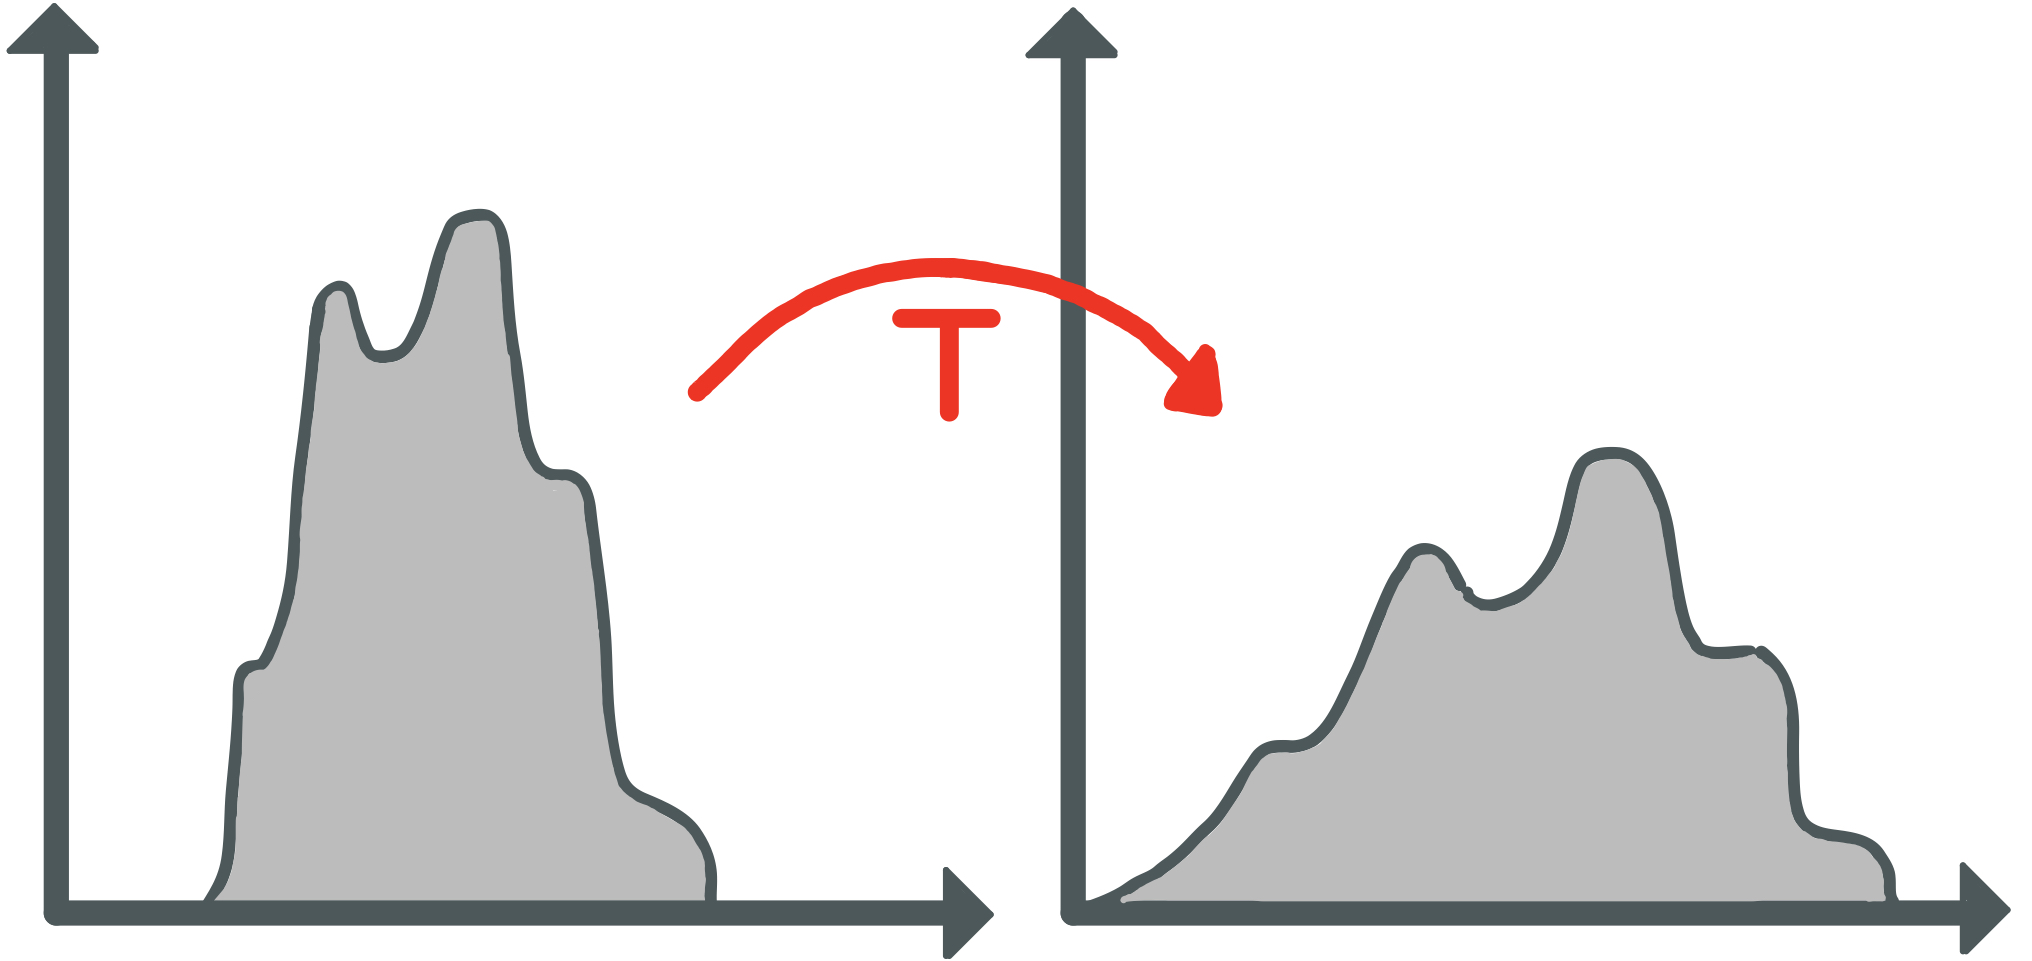
\includegraphics[scale = 0.08]{Figure/istogramma} %tra le graffe mettere il nome del file che va importato qui di fianco, sotto il main.tex
    \caption{Trasformazione dovuta all'equalizzazione}
    \label{istogramma}
\end{figure}

\subsection{Specifiche generali}
L'immagine è letta sequenzialmente da memoria, dove si trova memorizzata come mostrato in Figura \ref{elaboratore}. %In questa fase vengono calcolati dall'elaboratore i valori massimo e minimo di intensitá dei pixel che saranno poi utilizzati nella fase successiva.
Ogni pixel dell'immagine è trasformato per mezzo dell'algoritmo fornito e riscritto in memoria a partire dalla prima cella disponibile.

%piccolo esempio
Un esempio di funzionamento del componente è mostrato in Figura \ref{elaboratore} dove il blocco "Elaboratore" è quello realizzato dalla entity \texttt{"project\_reti\_logiche"}.
%In figura é possibile distinguere 3 tipologie differenti di frecce, alcune entranti nella macchina e altre uscenti. Le prime (frecce rosse) stanno ad indicare il flusso di dati in ingresso al componente una volta che quest'ultimo richiede alla memoria il contenuto di uno specifico indirizzo. Le frecce in blu rappresentano il flusso di dati in uscita dal componente una volta terminata la fase di modifica del pixel, questi vengono salvati in memoria specificando l'indirizzo nel quale si desidera memorizzare il dato. Infine la freccia nera consente di interagire con la memoria, in lettura e scrittura, andando a specificare di quale indirizzo si desidera sapere il contenuto o andare a memorizzare informazioni.
Il modulo comunica alla memoria gli indirizzi da cui vuole leggere o su cui vuole scrivere (freccia nera), legge il valore dei pixel (frecce rosse), applica l'algoritmo e scrive in uscita i valori sulla memoria (frecce blu).

L’indirizzo x rappresenta il primo indirizzo di memoria nel quale si andrá a memorizzare l’immagine.


%immagine
\begin{figure}[ht]
    \centering           %0.3
    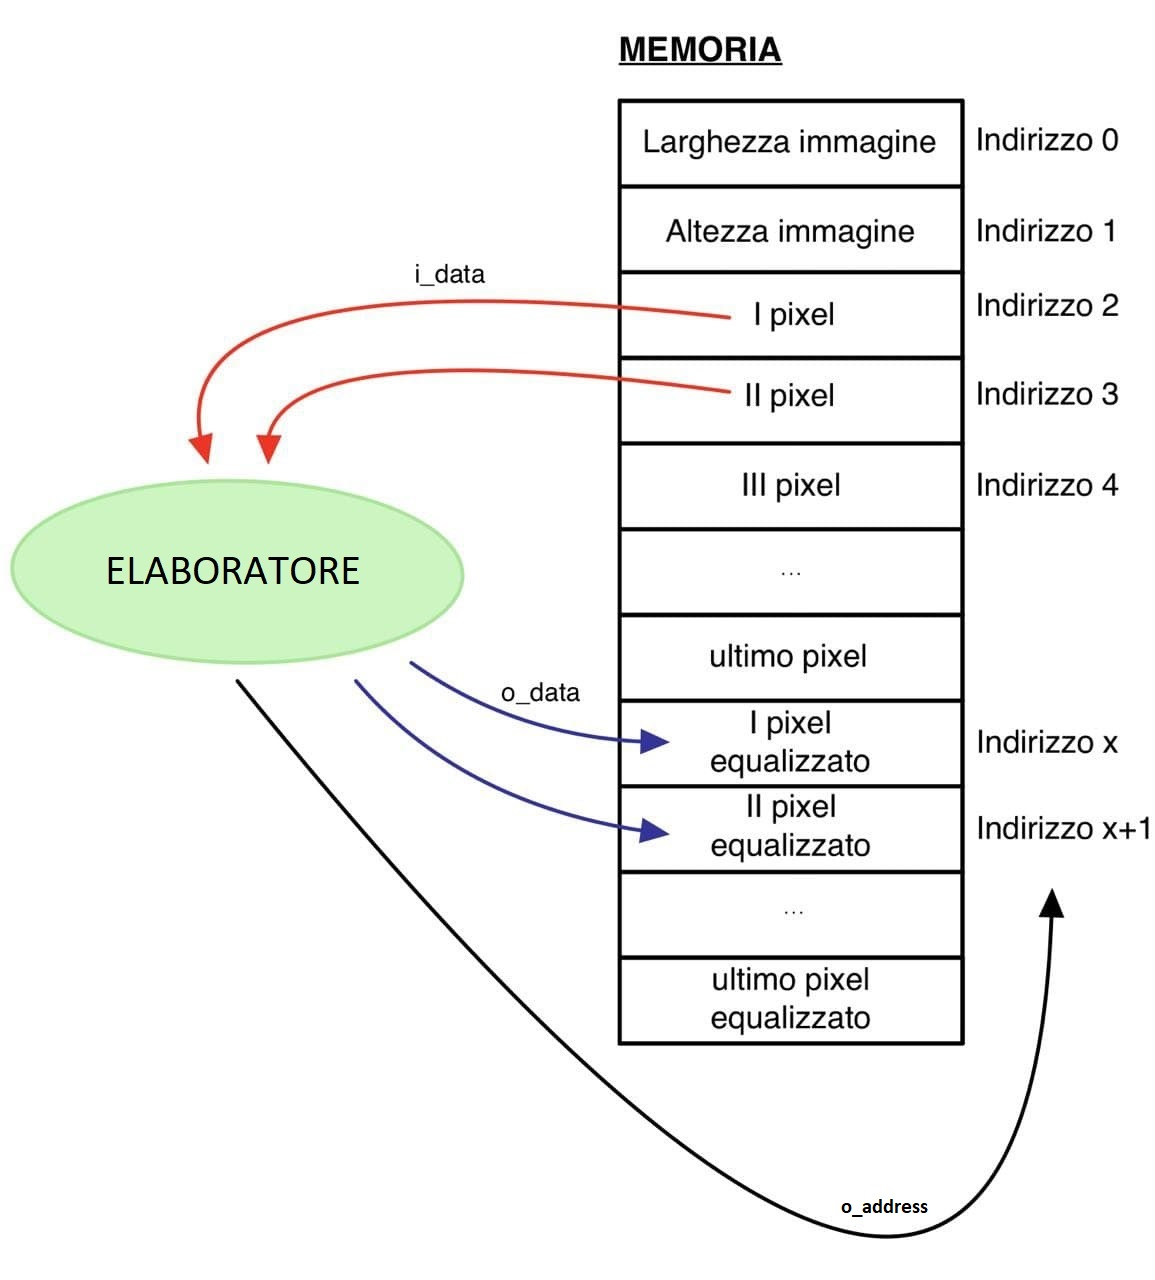
\includegraphics[scale = 0.205]{Figure/elaboratore} %tra le graffe mettere il nome del file che va importato qui di fianco, sotto il main.tex
    \caption{Funzionamento ad alto livello del componente (Elaboratore)}
    \label{elaboratore}
\end{figure}

\clearpage	
\section{Architettura}
%descrizione generale del progetto
Per la progettazione del componente si è scelto di utilizzare un architettura modulare divisa in un'unità di elaborazione (Data path) e un'unità di controllo (FSM).

Da un'ottica di alto livello, l'implementazione esegue i seguenti passi:
\begin{enumerate}
\item carico nel primo registro il valore della prima cella di memoria
\item carica nel secondo registro il valore della seconda cella di memoria
\item calcola la dimensione dell'immagine utilizzando un blocco che conta i pixel
\item legge 1 ad 1 tutti i pixel dell'immagine e ne calcola massimo e minimo
\item calcola il delta tra massimo e minimo, il log e lo shift\_level come da specifica
\item esegue lo shift e scrive a partire dal primo indirizzo di memoria libero i valori dei nuovi pixel, calcolati come da specifica calcolando MIN( 255 , TEMP\_PIXEL)
\end{enumerate}

Per la realizzazione del modulo sono stati utilizzati registri di tipo parallelo-parallelo che aggiornano il proprio contenuto sul fronte di salita del clock. 
Tutti i registri sono stati definiti in VHDL con approccio behaviuoral tramite Process e hanno tutti sensitivity list (i\_rst, i\_clk) e, in caso di reset (asincrono), vengono resettati al valore '0'.

%%%%%%%%%%%%
\subsection{Datapath}
In questa sezione è descritto il DataPath dividendone la trattazione in moduli logici dedicati ad eseguire specifici tasks.

\begin{enumerate}
\item calcolo dimensione immagine
\item gestione indirizzi
\item esecuzione algoritmo
\end{enumerate}

\subsubsection{Calcolo dimensione immagine} 
Questo modulo è composto da 2 registri, \texttt{registro\_1} e \texttt{registro\_2} (realizzati come specificato precedentemente) che memorizzano rispettivamente il primo e secondo Byte di memoria.
A seguire sono presenti un sommatore, un sottrattore, un comparatore e un registro (\texttt{regTS})  che combinati consentono di calcolare per somme successive il numero di pixel totali dell'immagine.

%, per mezzo di un algoritmo a somme successive,

 A cascata è presente un ulteriore sommatore che, alla fine del conteggio, incrementa di 1 il valore presente in \texttt{regTS}\footnote{\texttt{la sensitivity list}, a differenza degli altri registri, comprende anche il segnale \texttt{i\_start} per permettere la reinizializzazione di questo specifico registro ogni volta che viene sottoposta al modulo una nuova immagine}. Questo valore è infine salvato nel registro \texttt{reg sum\_1} che viene portato in ingresso ad un comparatore e ad un multiplexer usati, come descritto di seguito, nel modulo di gestione indirizzi.

%%%%%%%%%
In questo modulo vengono generati 3 segnali d'uscita: \texttt{finish}, \texttt{o\_end} e \texttt{CZ}. I primi 2 hanno lo scopo di gestire 2 dei casi limite (verranno approfinditi di seguito) mentre il terzo é utilizzato per notificare la conclusione del processo che permette di contare i pixel presenti nell'immagine.



\subsubsection{Gestione indirizzi}
La gestione degli indirizzi è realizzata mediante 2 cicli di conteggio e un multiplexer.
Un ciclo é adibito al conteggio degli indirizzi di lettura (quello che in Figura \ref{Datapath} comprende il \texttt{registro count}), l'altro agli indirizzi di scrittura (Figura \ref{Datapath} ciclo che comprende \texttt{reg sum\_2)}. Tramite il multiplexer si può decidere da quale dei 2 cicli attingere l'indirizzo da mandare alla memoria per mezzo del segnale \texttt{addr\_sel}.

\newpage

Il ciclo di conteggio degli indirizzi è composto di:
\begin{itemize}
\item un multiplexer per l'inizializzazione dei registri
\item un sommatore a 16 bit che incrementa di 1 l'indirizzo ogni volta che \texttt{rco\_load}='1' e \texttt{rsu\_load}='1' rispettivamente
\item un registro per memorizzare l'indirizzo
\end{itemize}

Il segnale \texttt{o\_end}, che consente di terminare la fase di lettura e passare a quella di elaborazione, viene alzato nel momento in cui l'indirizzo corrente diventa uguale a quello memorizzato nel registro \texttt{reg sum\_1}.

Tutti i multiplexer sono stati realizzati in VHDL utilizzando il costrutto with-select.


\subsubsection{Esecuzione algoritmo}
Questo terzo modulo é quello adibito all'esecuzione dell'algoritmo vero e proprio.

Massimo e minimo sono implementati mediante 1 comparatore, 2 multiplexer e 1 registro.
Il comparatore confronta ad ogni ciclo il valore in ingresso su i\_data con quello memorizzato nel registro max/min e se i\_data è rispettivamente maggiore/minore viene memorizzato nel registro corrispondente, altrimenti viene mantenuto il valore precedente.
Alla fine della lettura dell'intera immagine, nei due registri (\texttt{registro max} e \texttt{registro min}) avrò memorizzato massimo e minimo, pronti per essere utilizzati per i calcoli successivi.\\

Vengono poi calcolati:

\begin{enumerate}
    \item \texttt{DELTA\_VALUE = MAX\_PIXEL\_VALUE – MIN\_PIXEL\_VALUE};
    \item \texttt{Y = FLOOR(LOG2(DELTA\_VALUE +1))};
    \item \texttt{SHIFT\_LEVEL = (8 – Y)};
\end{enumerate}


Questa fase si conclude calcolando per ogni pixel:
\begin{enumerate}
    \item[4.]  \texttt{TEMP\_PIXEL = (CURRENT\_PIXEL\_VALUE - MIN\_PIXEL\_VALUE) << SHIFT\_LEVEL};
\end{enumerate}

e assegnando il nuovo valore ad esso nel seguente modo
\begin{enumerate}
    \item[5.]   \texttt{NEW\_PIXEL\_VALUE = MIN( 255 , TEMP\_PIXEL)};
\end{enumerate}





per poi infine scriverlo in memoria.\\

Considerando la limitatezza del loro codominio, le funzioni di floor\_log e shift ("<<") sono state realizzate mediante dei process che mappano in maniera diretta il valore d'ingresso sul corrispondente valore in uscita.

%immagine Datapath
\begin{figure}[ht]
    \centering
    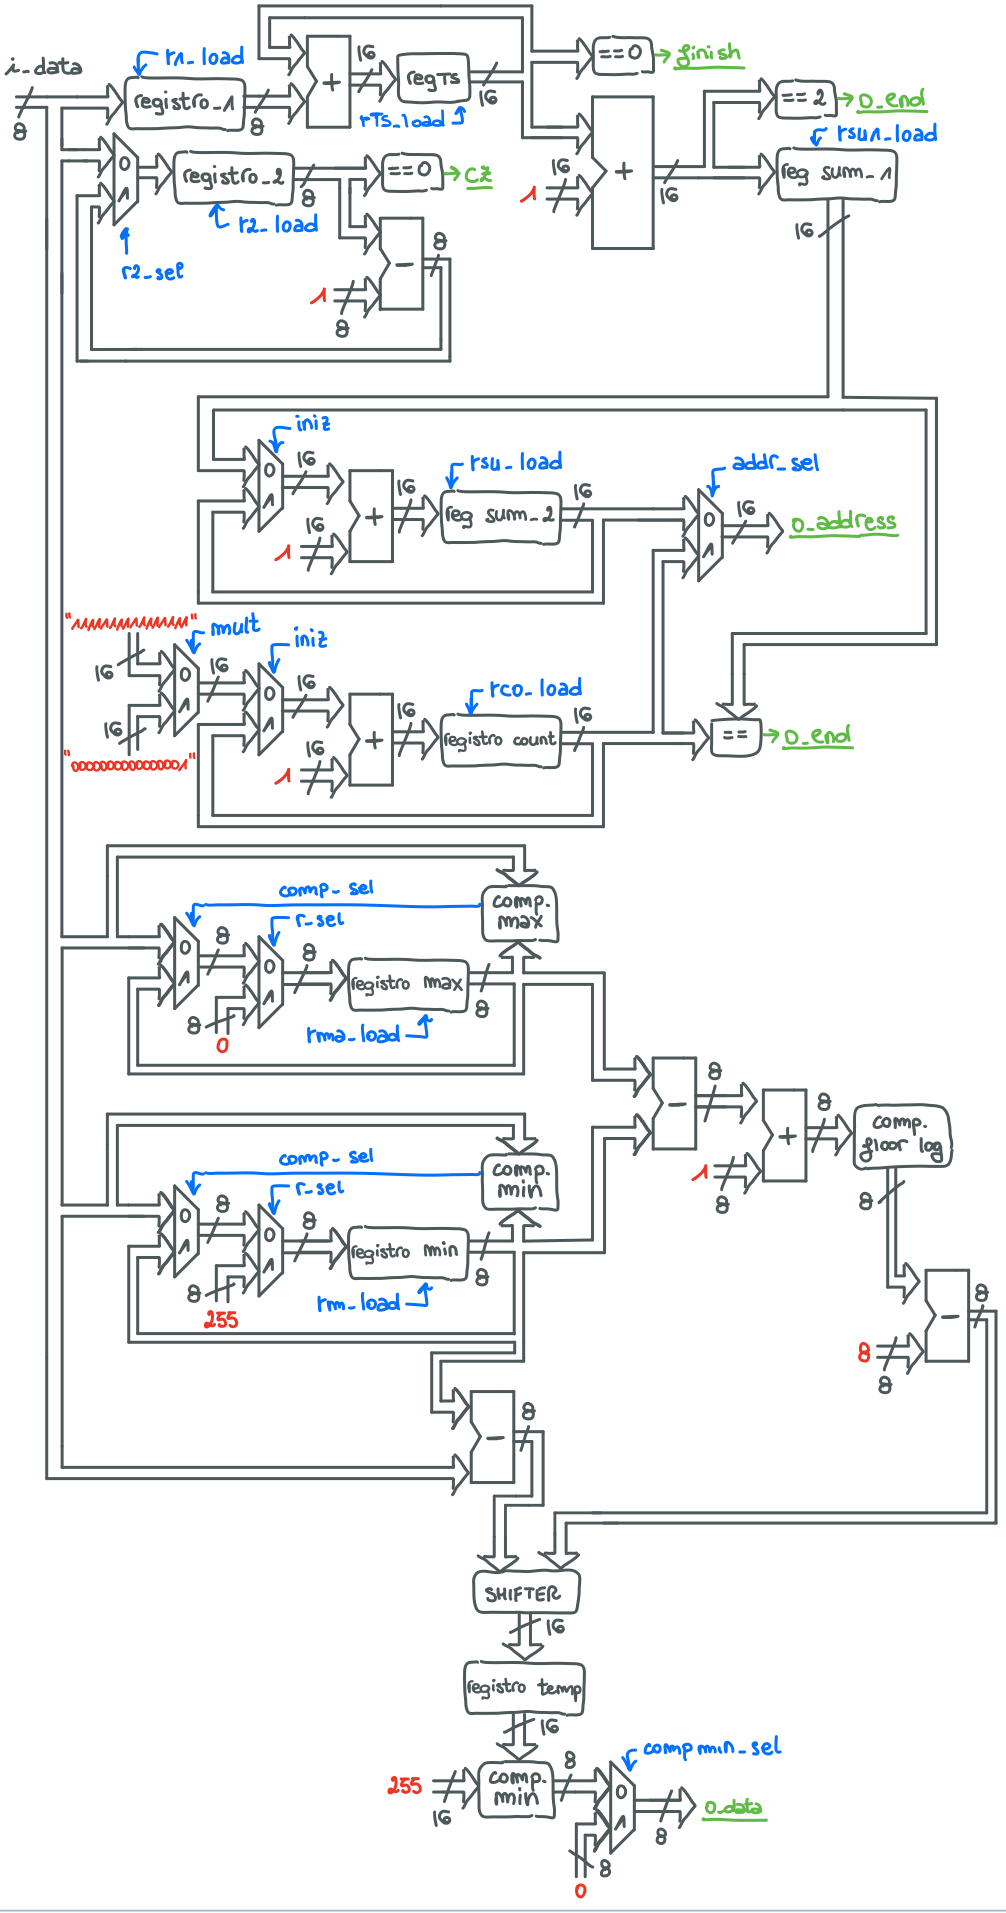
\includegraphics[scale = 0.34]{Figure/Datapath} 
    \caption{Datapath}
    \label{Datapath}
\end{figure}

\clearpage





\subsection{Macchina a Stati}

Si è scelto di utilizzare una sequenza di esecuzione separata per la gestione dei casi limite; questo per consentire il controllo di alcuni segnali parallelamente alla normale esecuzione, aumentandone la velocità nei suddetti casi. 

\begin{figure}[ht]
    \centering
    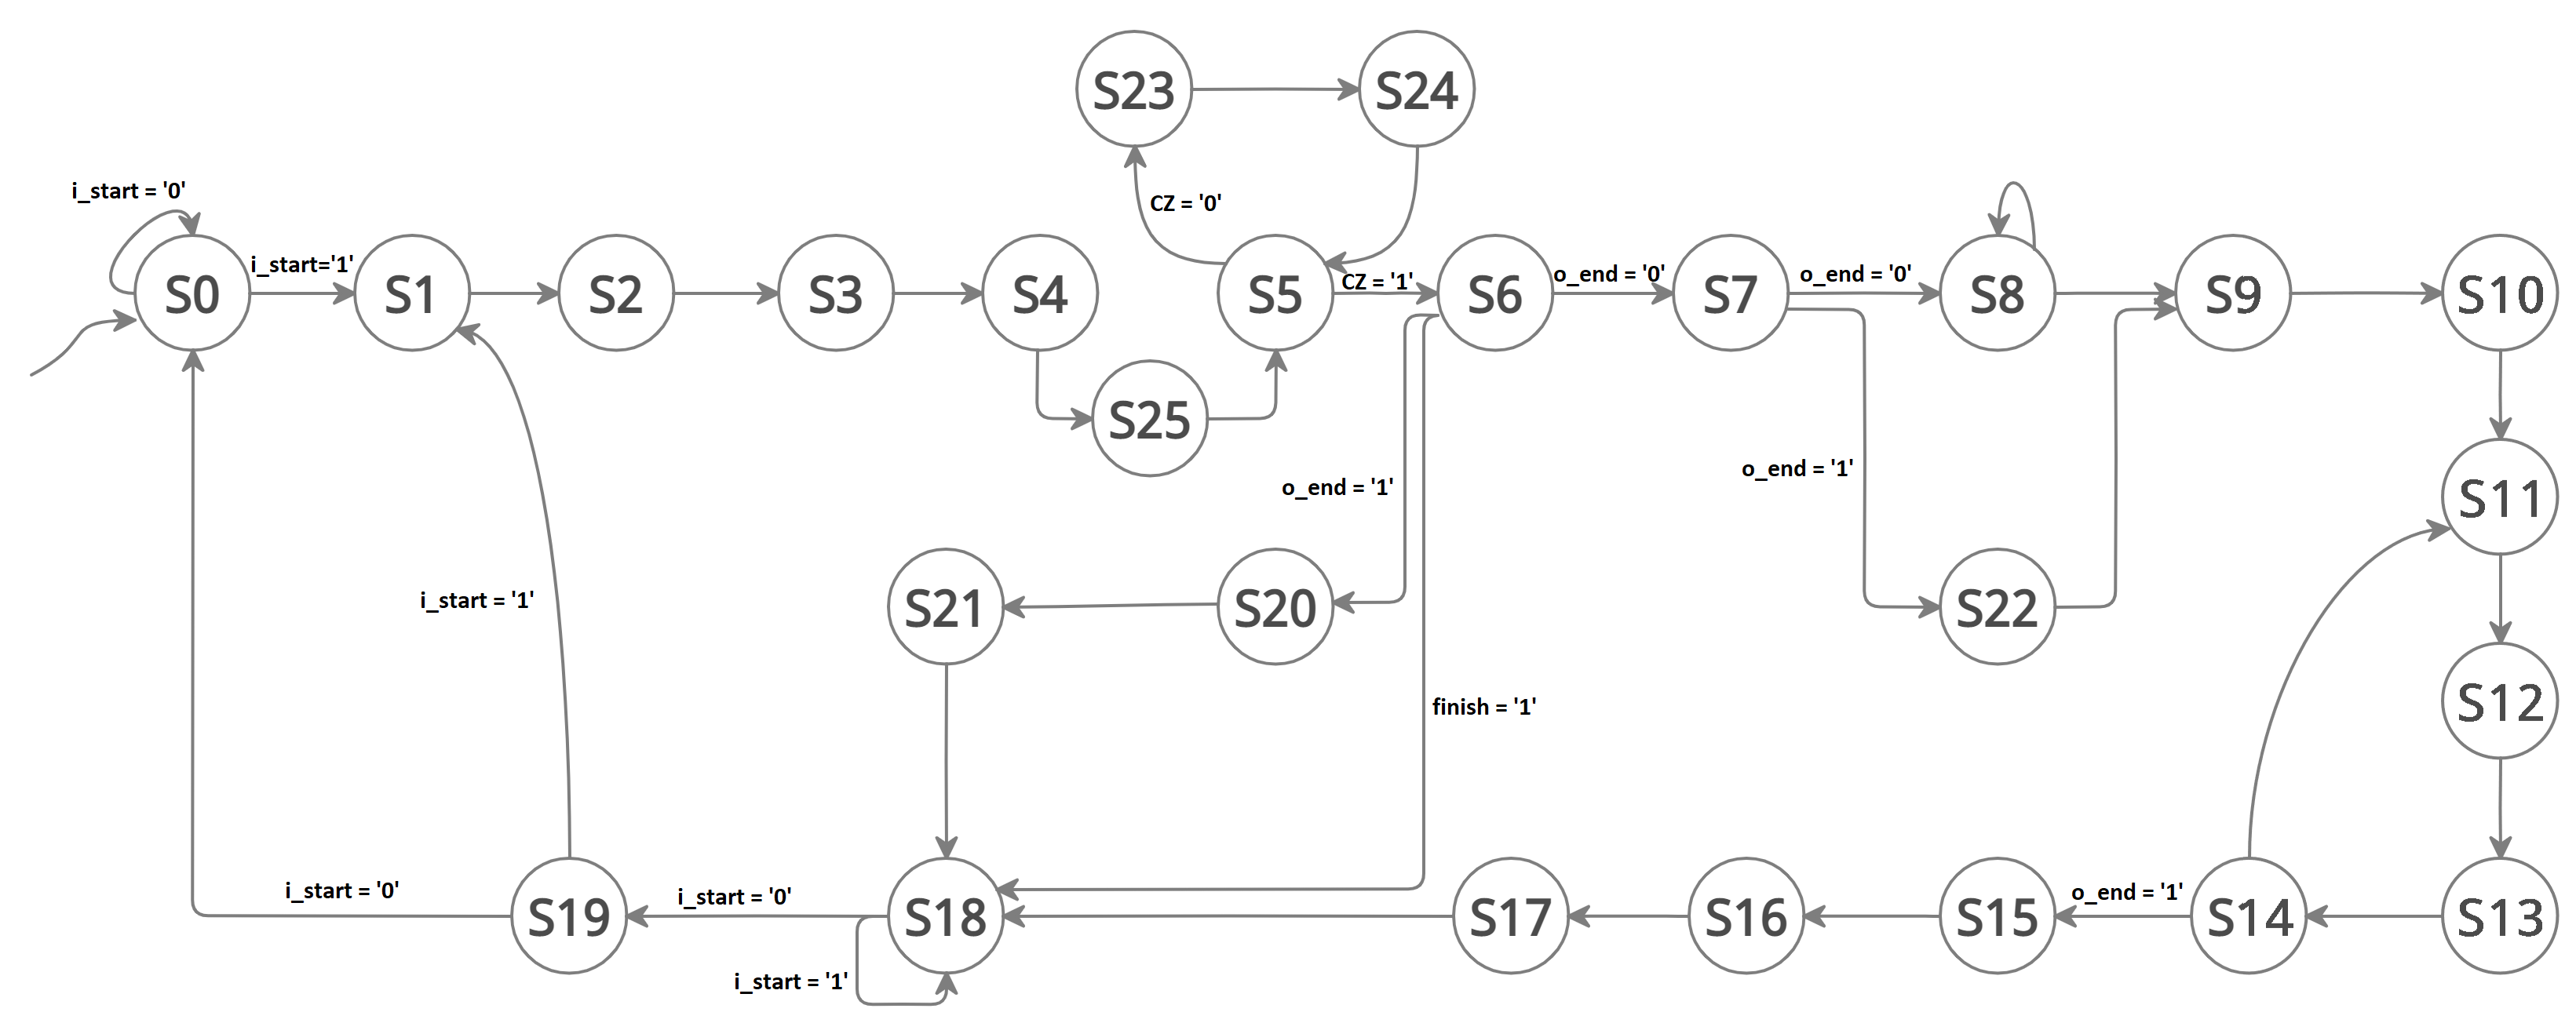
\includegraphics[scale = 0.182]{Figure/macchina a stati}
    \caption{Macchina a stati}
    \label{ms}
\end{figure}

\textit{\underline{oss}: E' stato assegnato il valore 0 come default a tutti i segnali della macchina a stati.}\\

Di seguito é riportata una breve descrizione per ogni stato della FSM:
\begin{itemize}
    \item[\textbf{S0}:]Stato di reset. Permette di attendere che l'equalizzazione abbia inizio. Si rimane in questo stato finché \texttt{i\_start} non viene alzato per passare quindi \textbf{S1};
    \item[\textbf{S1}:]Carica il registro \texttt{reg\_count} con il primo indirizzo di memoria ponendo \texttt{rco\_load}='1'; 
    \item[\textbf{S2}:]Inizializza il registro \texttt{reg\_max} a '0' e il registro \texttt{reg\_min} a '255'. Inoltre incrementa di 1 il valore memorizzato in \texttt{reg\_count} alzando il segnale \texttt{rco\_load} (quest'ultimo passaggio verrá ripetuto per incrementare gli indirizzi quando necessario);
    \item[\textbf{S3-S4}:] Consentono di immagazzinare il contenuto della prima e della seconda cella di memoria  rispettivamente nei registri \texttt{reg\_1} e \texttt{reg\_2}. Per farlo poniamo ad '1' i seguenti segnali: \texttt{r1\_load}, \texttt{r2\_load}, \texttt{o\_en}, \texttt{iniz}, \texttt{rco\_load};  

    \item[\textbf{S25}:]Introdotto per il corretto funzionamento del ciclo che permette di calcolare la dimensione dell'immagine. Consente al registro \texttt{reg2} di propagare il valore memorizzato nello stato precedente in uscita; 
    
    \item[\textbf{S5-S23-S24}:] Il ciclo composto da questi stati permette di calcolare il numero di pixel presenti nell'immagine. Viene portato avanti fino a che il contenuto del registro \texttt{reg\_2} é diverso da zero, appena questa condizione viene violata il segnale \texttt{CZ} viene alzato e da \textbf{S5} si passa ad \textbf{S6}. 
    Nel caso limite di immagini di dimensione 0 il segnale di controllo \texttt{CZ} é subito posto alto e dallo stato \textbf{S5} passo direttamente a \textbf{S6};
    
    \item[\textbf{S6}:] Lo stato piú importante dell'intera FSM; permette di individuare 2 dei 3 possibili casi limite, quello delle immagini con dimensione 0 e dimensione 1.
    Per prima cosa memorizza il valore dell'ultimo indirizzo di memoria da leggere in \texttt{reg sum\_1}, che consentirá (come descritto nel datapath) di terminare la lettura. 
    Avendo giá in questo stato a disposizione il valore del primo pixel in memoria, lo confronta con il valore contenuto nei registri max e min.
    
    In caso di una immagine di dimensione 0, avendo il segnale \texttt{finish}='1', passerei direttamente nello stato \textbf{S18}. 
    
    In caso invece di un'immagine di dimensione 1, avendo \texttt{o\_end}='1', percorrerei il ramo predisposto per questo caso specifico andando nello stato \textbf{S20};
    \item[\textbf{S7}:]Consente di individuare l'eventuale terzo caso limite(immagini di dimensione 2). In caso affermativo (se il segnale \texttt{o\_end} è alto) salto direttamente allo stato \textbf{S22};
    \item[\textbf{S8}:]Legge ciclicamente grazie all'auto-anello tutti i pixel dell'immagine salvando il loro valore, se necessario (vedi descrizione Datapath), nei registri \texttt{reg\_max} e \texttt{reg\_min}. Rimango in questo stato fino a che il segnale \texttt{o\_end} é tenuto basso;  
    \item[\textbf{S9}:]Terminata la lettura, in questo stato vengono inizializzati i registri che si occupano della memorizzazione degli indirizzi ai rispettivi valori iniziali. Per farlo occorre porre ad '1' i segnali \texttt{mult}, \texttt{rsu\_load}, \texttt{rco\_load};
    \item[\textbf{S10}:]Stato ponte che mi permette di attendere che sia disponibile il valore sull'uscita dei registri citati nello stato precedente;
    \item[\textbf{S11-S12-S13-S14}:] Il ciclo composto da questi stati é quello che ci permette di alternare l'output degli indirizzi (\texttt{o\_address}) usando il multiplexer comandato dal segnale \texttt{addr\_sel}. 
    Questo consente di alternare operazioni di scrittura e lettura.
    In caso di scrittura è fondamentale portare alti i segnali \texttt{o\_we} e \texttt{o\_address}.
    
    Se nello stato \textbf{S14} \texttt{o\_end} é alto, ovvero se siamo arrivati a leggere l'ultimo pixel dell'immagine, esco dal ciclo passando allo stato \textbf{S15};
    \item[\textbf{S15-S16-S17}:]Hanno il compito di completare elaborazione e scrittura in memoria dell'ultimo pixel. É stato necessario introdurre questi stati in quanto, per come é stato progettata la FSM, l'uscita dal ciclo sopra descritto avviene con la lettura dell'ultimo pixel dell'immagine;
    \item[\textbf{S18}:]Pone \texttt{o\_done}='1' e attende, con un auto-anello, che il segnale \texttt{i\_start} venga abbassato. Quando questo accade si passa allo stato \textbf{S19};   
    \item[\textbf{S19}:]Abbassa il segnale \texttt{o\_done} e a seconda che il segnale \texttt{i\_start} sia alto o basso (quindi a seconda che si voglia equalizzare subito un'altra immagine o meno) si passa rispettivamente negli stati \textbf{S1} o \textbf{S2};    
    \item[\textbf{S20-S21}:]Sequanza di stati che gestisce il caso particolare delle immagini di dimensione 1; 
    \item[\textbf{S22}:]Permette di gestire il caso particolare delle immagini di dimensione 2. 
\end{itemize}



\clearpage
\newpage
\section{Risultati Sperimentali}
\subsection{Sintesi}
Una volta eseguita la sintesi con successo sono stati analizzati 2 principali report:
\begin{itemize}
    \item \textbf{report\_timing} - risultati discussi nella Sezione \ref{Conclusione}
    \item \textbf{report\_utilization} - discusso di seguito
\end{itemize}

La rete ottenuta ha le seguenti caratteristiche: 
\begin{itemize}
    \item 138 Flip Flop - utilizzati per registri ad 8 e 16 bit e per memorizzare i 26 stati della macchina a stati con una codifica One-Hot
    \item  188 LUT
    \item  0 Latch - per evitare l'inferenza di Latch sono sempre stati inizializzati i segnali con un valore di default
\end{itemize}

Di seguito é riportato lo schema della rete realizzato da vivado:
%immagini
\begin{figure}[h!]
    \centering
    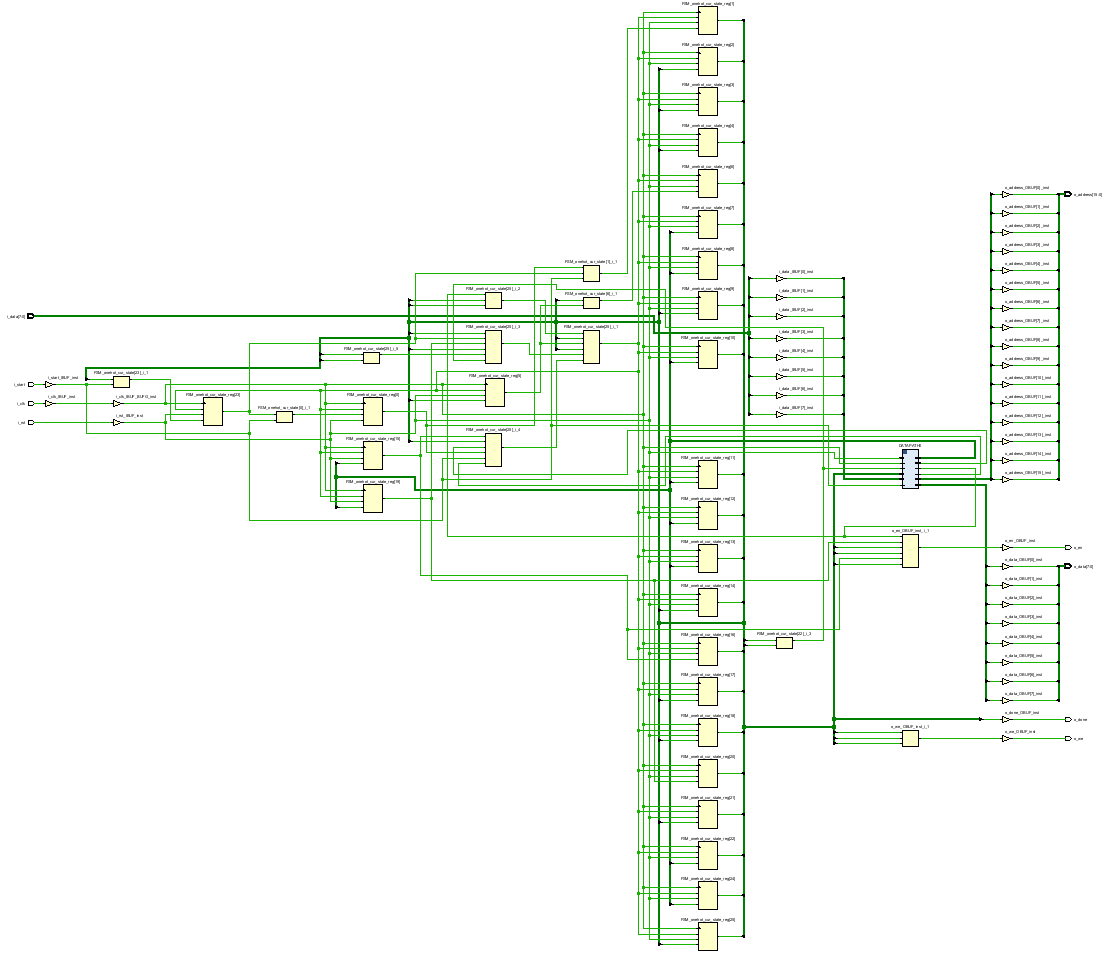
\includegraphics[scale = 0.54]{Figure/Sintesi}
    \caption{Schema del circuito sintetizzato}
    \label{Sintesi}
\end{figure}

\clearpage

\subsection{Simulazione}
Per verificare il corretto funzionamento del componente realizzato sono stati utilizzati diversi \textit{test bench} al fine di testare il comportamento, in Pre e Post sintesi, nella normale esecuzione e nei possibili casi limite.

Dopo aver appurato che il componente riuscisse a gestire semplici \textit{test bench} è stato sottoposto a 2 test per stressarne funzionalità e comportamento: 
\begin{itemize}
    \item il primo composto da una sequenza di 10 000 immagini di dimensione massima prefissata di 16 pixel per stressare il componente sotto il punto di vista dei reset;
    \item il secondo composto da una sequenza di 2000 immagini di dimensione massima prefissata di 128 pixel per stressare lettura e scrittura di grandi quantitá di dati in memoria e la gestione degli indirizzi in uscita.
\end{itemize}

I casi di test appena descritti hanno anche consentito di testare i casi limite, sia all'inizio del programma che all'interno di una serie di numerose altre operazioni, per assicurarsi della loro stabilità.

%%qui mettere una parte in cui descriviamo e mettiamo immagini di test di casi limite, immagini da 0 1 2 pixels
Abbiamo inoltre realizzato dei TB appositi per testare in maniera più specifica i casi limite di:
\begin{itemize}
    \item immagini di dimensione 0;
    \item immagini di dimensione 1;
    \item immagini di dimensione 2;
    \item immagini completamente bianche ;
    \item immagini completamente nere;
    \item immagini con pixel massimo '255' e pixel minimo '0' (con una conseguente non-necessità di equalizzare l'immagine);
\end{itemize}
che come spiegato in precedenza sono stati gestiti con un percorso di controllo alternativo della macchina a stati.

Di seguito riportiamo immagini e discussione di alcuni casi:
\subsubsection{Immagini di dimensione 0}

Nell'immagine (Figura \ref{0}) si può osservare che, come ci si aspetta, il segnale \texttt{finish} (che assume valore 0 solo nel momento in cui l'uscita di \texttt{registro\_TS} risulta essere != 0) rimane costante ad 1.
Questo consente di percorrere, partendo da S6, la sequenza di stati appositamente pensata per questo caso specifico.

\begin{figure}[h!]
    \centering
    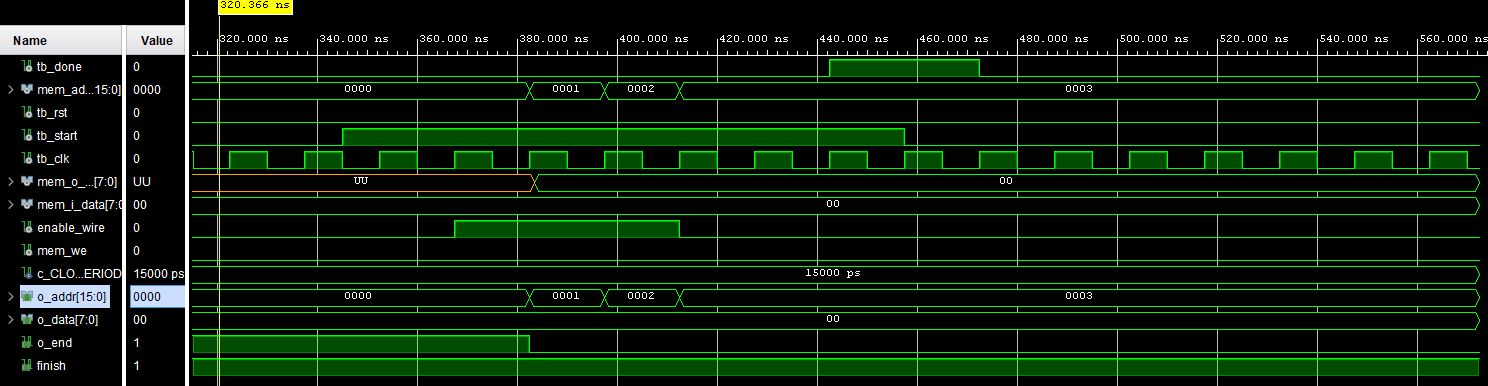
\includegraphics[scale = 0.3919]{Figure/TB_0x0.PNG}
    \caption{Screenshot caso particolare 1}
    \label{0}
\end{figure}

\clearpage

\subsubsection{Immagini di dimensione 1}
Nell'immagine (Figura \ref{1}) si può osservare che, appena dopo aver letto i primi 2 indirizzi di memoria e calcolato il numero di pixel, il segnale \texttt{o\_end} rimane alto (per via del comparatore che controlla che l'uscita di \texttt{regTS+1} sia uguale a 2) consentendo anche in questo caso di seguire il percorso di controllo dedicato. 


\begin{figure}[h!]
    \centering
    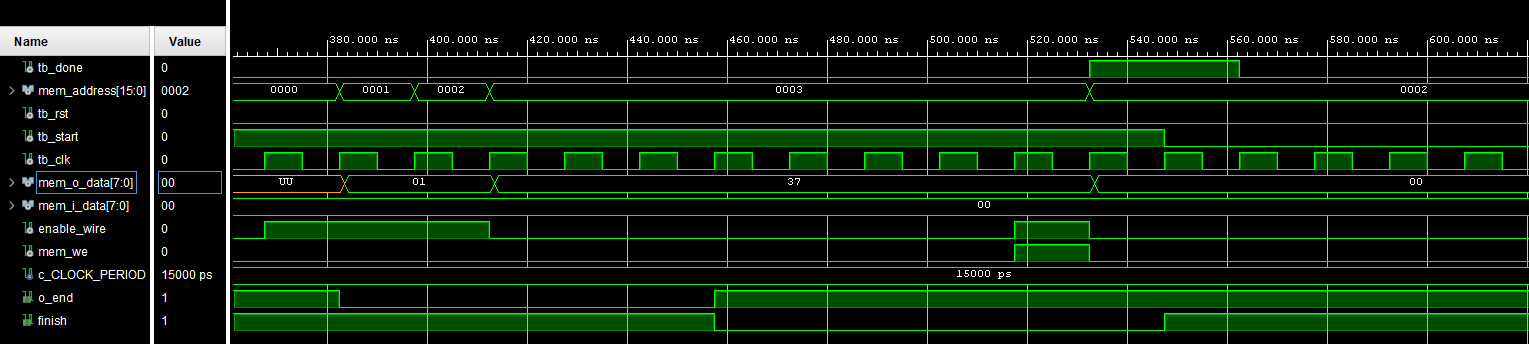
\includegraphics[scale = 0.3793]{Figure/TB_1x1.PNG}
    \caption{Screenshot caso particolare 2}
    \label{1}
\end{figure}

\subsubsection{Immagini di dimensione 2} %TODO

In questo ultimo caso (Figura \ref{2}) é possibile notare che il segnale \texttt{o\_end} viene portato alto prima rispetto al caso standard\footnote{\texttt{o\_end} viene posto a 1 almeno un ciclo di CK dopo la lettura del secondo pixel} in modo tale da evitare la lettura delle celle di memoria immediatamente successive (che sono le prime a non contenere l'immagine) per poi riabbassarlo e collegarsi al flow di controllo standard.
\begin{figure}[h!]
    \centering
    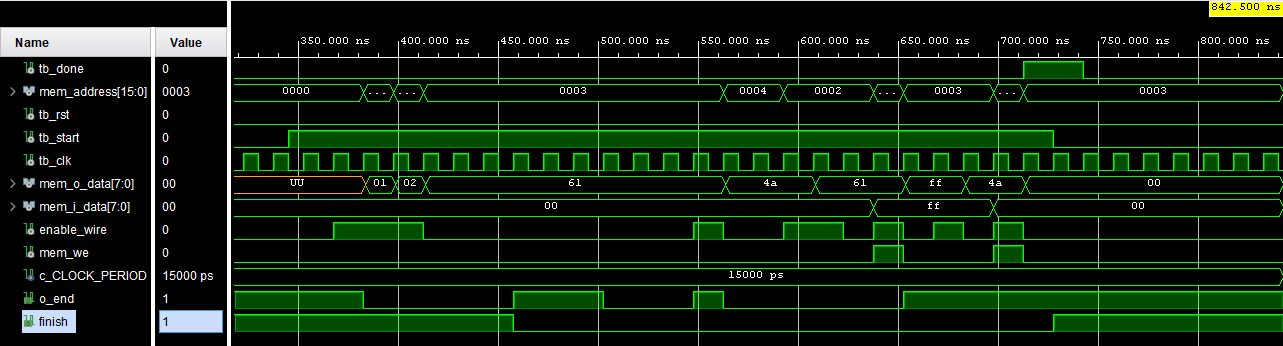
\includegraphics[scale = 0.45]{Figure/TB_2x1.PNG}
    \caption{Screenshot caso particolare 3}
    \label{2}
\end{figure}

\clearpage

\newpage
\section{Conclusioni}
\label{Conclusione}
É stato osservato che il componente si comporta in maniera corretta dopo averlo sottoposto ad una notevole quantitá di casi di test, sia in simulazioni Pre-Synthesis che in Functional-Post-Synthesis. Possiamo quindi supporre con buon livello di confidenza che il componente è esente da errori di natura progettuale.

Abbiamo inoltre analizzato il report temporale prodotto dalla Post-Synthesis osservando i seguenti risultati:

\begin{itemize}
    \item Data Path Delay:  5.304 [ns]   (37.406\% Logico e 62.594\% di Routing)
    \item Requirement:  100.000 [ns] 
    \item Slack (MET):  94.545 [ns] 
\end{itemize}

Dai dati sopra riportati ci é possibile dedurre che il componente potrebbe funzionare ad una frequenza decisamente maggiore rispetto a quella imposta in quanto lo Slack compone la quasi totalitá del ciclo di clock.
É stato possibile ottenere questo risultato optando per una soluzione con un maggior numero di registri; questo ha permesso di suddividere le operazioni su più cicli di clock, consentendo dunque di ridurre il tempo di lavoro nel singolo ciclo del componente.





\newpage
%%% Appendici %%%
% Eventuali appendici vanno qui. Se non avete appendici da inserire, togliete/commentate queste righe.
%\appendix
%\input{Sezioni/Appendice.tex}	

\end{document}

% Credits: basato sulle relazioni di laboratorio